\documentclass{article}
\usepackage{preamble}

\title{Software Assignment: Eigenvalue Calculation}
\author{AI24BTECH11031 - Shivram S}
\date{}

\begin{document}

\twocolumn
\maketitle
\tableofcontents

\section{Abstract}

\em
The computation of eigenvalues is a fundamental task in various fields. Eigenvalues
help us understand the behaviour of systems and reveal key information about the
properties of linear transformations.

This report discusses various algorithms to
compute the eigenvalues of a matrix, focusing on the QR algorithm, and discusses its
computational complexity, numerical stability, and suitability for different kinds of
matrices. Implementations of the algorithms are also presented.
\em

\section{Eigenvectors and Eigenvalues}

The eigenvectors of a matrix are vectors which do not change direction when transformed
by the matrix. That is, for a matrix $\vec{M}$, its eigenvectors are solutions to the
equation

\begin{align}    
\vec{M}\vec{p} = \lambda\vec{p}
\end{align}


$\vec{p}$ is the eigenvector, and the scalar $\lambda$ is called the eigenvalue.
If $\vec{M}$ is not a square matrix, then for any vector $\vec{v}$, $\vec{M}\vec{v}$
will not have the same dimension as $\vec{v}$. Hence, a non-square matrix does not have
any eigenvectors or eigenvalues.

For a square matrix, we may rewrite the above equation as
\begin{align}
(\vec{M} - \lambda\vec{I})\vec{p} = 0
\end{align}

If $\vec{p}$ is nonzero, then we can say that
\begin{align}
\abs{\vec{M} - \lambda\vec{I}} = 0
\end{align}

For an $n \times n$ matrix, the above determinant can be expanded to an $n^{th}$ degree
polynomial in $\lambda$. The solutions of this polynomial are the eigenvalues of the matrix.
The polynomial always has $n$ roots in the complex plane, counting multiplicities. For real
matrices, the complex eigenvalues always appear in conjugate pairs.

\section{Algorithm Selection}

There are several algorithms that can be used to calculate the eigenvalues of a matrix.
Some of these algorithms are listed below.

\begin{table}[h!]
    \centering
    \begin{tabular}{|c|p{6cm}|}
    \hline
    \textbf{Algorithm}        & \textbf{Description} \\
    \hline
    Power Iteration           & Iteratively finds the largest eigenvalue by repeatedly multiplying the matrix with a vector. \\
    \hline
    Inverse Iteration         & Finds the smallest eigenvalue by inverting the matrix and applying power iteration. \\
    \hline
    QR Algorithm              & Uses QR decomposition iteratively to compute all eigenvalues of a matrix. \\
    \hline
    Lanczos Algorithm         & Reduces a large sparse symmetric matrix to tridiagonal form for eigenvalue computation. \\
    \hline
    Arnoldi Iteration         & Generalizes the Lanczos method for non-symmetric matrices to compute a few eigenvalues. \\
    \hline
    Jacobi Method             & Rotates pairs of rows and columns to diagonalize the matrix iteratively. \\
    \hline
    Davidson Algorithm        & Specialized for large sparse matrices, builds a subspace to approximate eigenvalues. \\
    \hline
    \end{tabular}
    \caption{Eigenvalue Calculation Algorithms and Their Descriptions}
    \label{tab:eigenvalue_algorithms}
\end{table}
    

Methods such as Divide and Conquer or the Jacobi Method are applicable only for symmetric
matrices. Other algorithms such as the Davidson Algorithm and Arnoldi Iteration only compute a
small set of eigenvalues.

If we wish to compute all the eigenvalues of a $n \times n$ matrix, the
QR algorithm is the preferred due to its reliability and its ability
to find all eigenvalues for an arbitrary matrix.

\section{QR Algorithm}

The QR Algorithm is an iterative algorithm which starts with a matrix $\vec{A_0} \coloneqq \vec{A}$,
and then calculates the iterative result $\vec{A_{k+1}}$ by first decomposing $\vec{A_k}$ as the
product of an orthogonal matrix $\vec{Q}_k$ and an upper-triangular matrix $\vec{R}_k$ such that
\begin{align}
\vec{A_k} = \vec{Q_k}\vec{R_k}
\end{align}

and then using $\vec{Q_k}$ and $\vec{R_k}$ to compute $\vec{A_{k+1}} = \vec{R_k} \vec{Q_k}$.
This process is repeated until the result converges to an upper-triangular matrix, in which
case the eigenvalues are given by the diagonal elements.

The QR algorithm works on the principle of matrix similarity. Two matrices are
similar if they represent the same transformation but in different bases. That is,
if two matrices $\vec{A}$ and $\vec{B}$ are similar, then there exists some invertible
matrix $\vec{P}$ (called the change-of-basis matrix) such that
\begin{align}
\vec{B} = \vec{P^{-1}}\vec{A}\vec{P}
\end{align}

We can show that $\vec{A_{k+1}}$ and $\vec{A_k}$ are similar matrices, and thus have the 
same eigenvalues.
\begin{align}
    \vec{A_{k+1}} &= \vec{R_k}\vec{Q_k} \\
    &= \vec{Q_k^{-1}}\vec{Q_k}\vec{R_k}\vec{Q_k} \\
    &= \vec{Q_k^{-1}}\vec{A_k}\vec{Q_k}
\end{align}

$\vec{Q_k}$ is invertible because it is orthogonal ($\vec{Q_k^{-1}} = \vec{Q}^\top$).

The QR decomposition of any matrix $\vec{M}$ can be done in multiple ways.

\subsection{Using the Gram-Schmidt process}

The Gram-Schmidt process is used to construct an orthonormal basis from a set of
vectors. We first define the projection of a vector $\vec{v}$ along a vector $\vec{u}$
as 
\begin{align}
    \proj_{\vec{u}}(\vec{v}) = \frac{\vec{u} \cdot \vec{v}}{\vec{u} \cdot \vec{u}} \vec{u}
\end{align}

Subtracting the projection of $\vec{v}$ along $\vec{u}$ from $\vec{v}$ gives us a vector
which is orthogonal to $\vec{u}$. We can verify this by showing that their dot product
is zero.

\begin{align}
    (\vec{v} - \proj_{\vec{u}}(\vec{v})) \cdot \vec{u} &= \vec{v} \cdot \vec{u} - \proj_{\vec{u}}(\vec{v}) \cdot \vec{u} \\
    &= \vec{u} \cdot \vec{v} - \frac{\vec{u} \cdot \vec{v}}{\vec{u} \cdot \vec{u}} (\vec{u} \cdot \vec{u}) \\
    &= \vec{u} \cdot \vec{v} - \vec{u} \cdot \vec{v} \\
    &= 0
\end{align}

Given a set of vectors $\vec{v_1}, \vec{v_2}, \dots, \vec{v_n}$, the Gram-Schmidt process
gives us a set of orthogonal vectors $\vec{u_1}, \vec{u_2}, \dots, \vec{u_n}$ as follows: 
\begin{align}
    \vec{u_1} &= \vec{v_1} \\
    \vec{u_2} &= \vec{v_2} - \proj_{\vec{u_1}}(\vec{v_2}) \\
    \vec{u_3} &= \vec{v_3} - \proj_{\vec{u_1}}(\vec{v_3}) - \proj_{\vec{u_2}}(\vec{v_3}) \\
    \vdots \\
    \vec{u_k} &= \vec{v_k} - \sum_{j=1}^{k-1} \proj_{\vec{u_j}}(\vec{v_k})
\end{align}

We can then normalize these vectors to obtain a set of orthonormal vectors
$\vec{e_1}, \vec{e_2}, \dots, \vec{e_n}$ where
\begin{align}
    \vec{e_k} = \frac{\vec{u_k}}{\norm{\vec{u_k}}}
\end{align}

We can express this in pseudocode as 

\begin{algorithm}
\Begin{
    \For{$i \gets 1$ \KwTo $n$}{
        $\vec{u}[i] \gets \vec{v}[i]$\;
        \For{$j \gets 1$ \KwTo $(i-1)$}{
            $\vec{u}[i] \gets \vec{u}[i] - \proj(\vec{u}[j], \vec{v}[i])$\;
        }
    }
    \For{$i \gets 1$ \KwTo $n$}{
        $\vec{e}[i] = \vec{u}[i] / \norm{\vec{u}[i]}$\;
    }
    \caption{Gram-Schmidt Process}
}
\end{algorithm}

Given an $n \times n$ matrix $\vec{A}$, we can construct the vectors
$\vec{v_1}, \dots, \vec{v_n}$ from the columns of the matrix. That is,
\begin{align}
    \vec{A} = \mat{\vec{v_1} & \vec{v_2} & \dots & \vec{v_n}}
\end{align}

We can apply the Gram-Schmidt procedure to get the orthogonal matrix
\begin{align}    
\vec{Q} = \mat{\vec{e_1} & \vec{e_2} & \dots & \vec{e_n}}
\end{align}

Since the vectors $\vec{e_1}, \dots, \vec{e_n}$ are orthonormal, we can
write each column of $\vec{A}$ in terms of the orthonormal basis as
\begin{align}
\vec{v_1} &= (\vec{e_1} \cdot \vec{v_1}) \vec{e_1} \\
\vec{v_2} &= (\vec{e_1} \cdot \vec{v_2}) \vec{e_1} + (\vec{e_2} \cdot \vec{v_2}) \vec{e_2} \\
\vdots \\
\vec{v_k} &= \sum_{i=1}^k (\vec{e_i} \cdot \vec{v_k}) \vec{e_i}
\end{align}

Thus, the matrix $\vec{R}$ is
\begin{align}
    \vec{R} = \mat{
        \vec{e_1} \cdot \vec{v_1} & \vec{e_1} \cdot \vec{v_2} & \dots  & \vec{e_1} \cdot \vec{v_n} \\
        0                         & \vec{e_2} \cdot \vec{v_2} & \dots  & \vec{e_2} \cdot \vec{v_n} \\
        \vdots                    & \vdots                    & \ddots & \vdots                    \\
        0                         & 0                         & \dots  & \vec{e_n} \cdot \vec{v_n}
    }
\end{align}

Thus, the matrix $\vec{A}$ has been decomposed to $\vec{Q}\vec{R}$, where $\vec{Q}$ is
an orthogonal matrix and $\vec{R}$ is an upper-triangular matrix.

\subsubsection{Modified Gram-Schmidt process}

When performing the Gram-Schmidt process, we calculate each orthogonal vector $\vec{u_k}$ as 
\begin{align}
    \vec{u_k} = \vec{v_k} - \sum_{j=1}^{k-1} \proj_{\vec{u_j}}(\vec{v_k})
\end{align}

This method, called the Classical Gram-Schmidt, accumulates numerical errors
during the projection step, due to which the final result may not be exactly
orthogonal. To avoid these errors, we sequentially orthonormalize each vector
instead of summing the projections:
\begin{align}
    \vec{u_k}^{(0)} &= \vec{v_k} \\
    \vec{u_k}^{(1)} &= \vec{u_k}^{(0)} - \proj_{\vec{u_1}}\brak{\vec{u_k}^{(0)}} \\
    \vdots \\
    \vec{u_k}^{(k)} &= \vec{u_k}^{(k-1)} - \proj_{\vec{u_{k-1}}}\brak{\vec{u_k}^{(k-1)}} \\
\end{align}

The final result $\vec{u_k}^{(k)}$ is more numerically stable and orthogonal than the results
produced by Classical Gram-Schmidt.

\subsection{Using Householder transformations}

A Householder transformation describes a reflection about a hyperplane containing the origin.
Each hyperplane can be defined by its normal vector, $\vec{v}$, and the
reflection of any vector $\vec{x}$ about this hyperplane is given by
\begin{align}
    \vec{x^\prime} = \vec{x} - 2(\vec{v} \cdot \vec{x})\vec{v}
\end{align}

This transformation can be expressed in matrix form as
\begin{align}
    \vec{H} = \vec{I} - 2\frac{\vec{v}\vec{v}^\top}{\vec{v}^\top\vec{v}}
\end{align}

We can verify that the Householder matrix is an orthogonal matrix
\begin{align}
    \vec{H}^\top\vec{H} &= \brak{\vec{I} - 2\frac{\vec{v}\vec{v}^\top}{\vec{v}^\top\vec{v}}}^\top\brak{\vec{I} - 2\frac{\vec{v}\vec{v}^\top}{\vec{v}^\top\vec{v}}} \\
    &= \brak{\vec{I}^\top - 2\frac{\brak{\vec{v}\vec{v}^\top}^\top}{\vec{v}^\top\vec{v}}}\brak{\vec{I} - 2\frac{\vec{v}\vec{v}^\top}{\vec{v}^\top\vec{v}}} \\
    &= \brak{\vec{I} - 2\frac{\vec{v}\vec{v}^\top}{\vec{v}^\top\vec{v}}}\brak{\vec{I} - 2\frac{\vec{v}\vec{v}^\top}{\vec{v}^\top\vec{v}}} \\
    &= \vec{I}^2 - 4\frac{\vec{v}\vec{v}^\top}{\vec{v}^\top\vec{v}} + 4\brak{\frac{\vec{v}\vec{v}^\top}{\vec{v}^\top\vec{v}}}^2 \\
    &= \vec{I} - 4\frac{\vec{v}\vec{v}^\top}{\vec{v}^\top\vec{v}} + 4\frac{\vec{v}\vec{v}^\top}{\vec{v}^\top\vec{v}} \\
    &= \vec{I}
\end{align}

To transform $\vec{A}$ into an upper-triangular matrix we have to compute Householder
matrices that, when applied to $\vec{A}$, will zero out elements below the
principal diagonal. For each column vector of $\vec{A}$, we consider the subvector
of elements starting from the principal diagonal.

\begin{figure}[h!]
\centering
\begin{tikzpicture}
    \matrix(m)[matrix of math nodes,left delimiter=(,right delimiter=)] {
        1 & 2 & 3 & 4 \\
        5 & 6 & 7 & 8 \\
        9 & 10 & 11 & 12 \\
        13 & 14 & 15 & 16 \\
    };
    \draw (m-1-1.north west) rectangle (m-4-1.south east);
    \draw (m-4-1.south) node[below] {$\vec{u_1}$};
    \draw (m-2-2.north west) rectangle (m-4-2.south east);
    \draw (m-4-2.south) node[below] {$\vec{u_2}$};
    \draw (m-3-3.north west) rectangle (m-4-3.south east);
    \draw (m-4-3.south) node[below] {$\vec{u_3}$};
    \draw (m-4-4.north west) rectangle (m-4-4.south east);
    \draw (m-4-4.south) node[below] {$\vec{u_4}$};
\end{tikzpicture}
\end{figure}

\pagebreak

For each subvector $\vec{u_i}$, we have to construct a Householder
matrix that zeroes out all components except the first component.
We can do this by reflecting the vector onto the $x$-axis.

\begin{figure}[h!]
\centering
\begin{tikzpicture}
    \draw[->] (0, 0) node[below] {$O$} -- (1, 1.73) node[above] {$\vec{u_i}$};
    \draw[<->] (-2, 0) node[left] {$\vec{x}^\prime$} -- (2, 0) node[right] {$\vec{x}$};
    \draw[dashed] (-1.73, -1) -- (1.73, 1);
\end{tikzpicture}
\end{figure}

The normal to the hyperplane, $\vec{v}$ is given by
\begin{align}
    \vec{v_i} = \vec{u_i} - \norm{\vec{u_i}} \vec{e_1}
\end{align}

The constructed Householder matrix $\vec{H_{sub}}$ is of order $(n-i+1) \times (n-i+1)$.
To facilitate multiplication with the matrix $\vec{A}$, we extend the matrix as
\begin{align}
    \vec{H_i} = \mat{\vec{I} & \vec{0} \\ \vec{0} & \vec{H_{sub}}}
\end{align}

We can now write obtain the upper-triangular matrix $\vec{R}$:
\begin{align}
    \vec{R} = \vec{H_1} \vec{H_2} \dots \vec{H_n} \vec{A}
\end{align}

and the orthogonal matrix $\vec{Q}$ is given by
\begin{align}
    \vec{Q} &= \vec{H_n}^\top \vec{H_{n-1}}^\top \dots \vec{H_1}^\top \\
    &= \vec{H_n} \vec{H_{n-1}} \dots \vec{H_1}
\end{align}

It can be easily verified that $\vec{A} = \vec{Q}\vec{R}$
\begin{align}
    \vec{Q}\vec{R} &= \Big( \vec{H_n}^\top \dots \vec{H_1}^\top \Big) \Big( \vec{H_1}\dots\vec{H_n}\vec{A} \Big) \\ 
    &= \vec{H_n}^\top \dots \vec{H_1}^\top\vec{H_1} \dots \vec{H_n} \vec{A} \\
    &= \vec{H_n}^\top \dots \vec{H_2}^\top\vec{H_2} \dots \vec{H_n} \vec{A} \\
    &\vdots \\
    &= \vec{A}
\end{align}

Thus, the matrix $\vec{A}$ has been decomposed to $\vec{Q}\vec{R}$, where $\vec{Q}$ is
an orthogonal matrix and $\vec{R}$ is an upper-triangular matrix.

The algorithm has been expressed in pseudocode in [Algorithm 2].

\begin{algorithm}
\Begin{
    $\vec{Q} \gets \vec{I}_{n \times n}$\;
    $\vec{R} \gets \vec{A}$\;
    \For {$i \gets 1$ \KwTo $n$} {
        $\vec{u_i} \gets \vec{A}[i:, i]$\;
        $\vec{v_i} \gets \vec{u_i} - \norm{\vec{u_i}}\vec{e_1}$\;
        $\vec{H_{sub}} \gets \vec{I} - 2\frac{\vec{v}\vec{v}^\top}{\vec{v}^\top\vec{v}}$\;
        $\vec{H_i} \gets \mat{\vec{I} & \vec{0} \\ \vec{0} & \vec{H_{sub}}}$\;
        $\vec{Q} \gets \vec{Q}\vec{H_i}$\;
        $\vec{R} \gets \vec{H_i}\vec{R}$\;
    }
    \caption{QR Decomposition using Householder Transformations}
} 
\end{algorithm}


\section{Generalization}

The algorithms described above works for real-valued matrices which have real 
eigenvalues. To extend the algorithm to real-valued matrices with complex eigenvalues,
and to complex matrices, slight modifications need to be made to the algorithm.

\subsection{Complex eigenvalues - quasi-triangular matrices}

If a real matrix has complex eigenvalues, then QR algorithm converges to an 
upper quasi-triangular matrix rather than an upper-triangular matrix. In an upper
quasi-triangular matrix, the entries below the first subdiagonal are zero. The below
matrix is an example.
\begin{align}
    \mat{
        1 & 2 & 3 & 4 \\
        5 & 6 & 7 & 8 \\
        0 & 9 & 10 & 11 \\
        0 & 0 & 12 & 13
    }
\end{align}

To find the eigenvalues of a quasi-triangular matrix, we move along the diagonal.
If the subdiagonal element to the right of a particular diagonal element is
zero, then the diagonal element is an eigenvalue of the matrix.

If the subdiagonal element is non-zero, then we consider a $2 \times 2$ block
with the top-left corner at the diagonal element, and derive a pair of
eigenvalues from it.

\begin{figure}[h!]
\centering
\begin{tikzpicture}
    \matrix(m)[matrix of math nodes,left delimiter=(,right delimiter=)] {
        2 & 0 & 0 & 0 \\
        0 & 1 & 2 & 0 \\
        0 & -2 & 1 & 0 \\
        0 & 0 & 0 & 1 \\
    };
    \draw[dashed] (m-1-1.north west) rectangle (m-1-1.south east);
    \draw[dashed] (m-2-2.north west) rectangle (m-3-3.south east);
    \draw[dashed] (m-4-4.north west) rectangle (m-4-4.south east);
\end{tikzpicture}
\end{figure}

The above $4 \times 4$ Hessenberg matrix gives us two eigenvalues 2 and 1,
and a $2 \times 2$ block $\mat{1 & -2 \\ 2 & 1}$. For a block $\vec{B}$,
we can write the eigenvalue equation as
\begin{gather}
    \det{\vec{B} - \lambda\vec{I}} = 0 \\ 
    \lambda^2 - \tr(\vec{B})\lambda + |\vec{B}| = 0 \\
    \lambda = \frac{\tr(\vec{B})}{2} \pm \frac{1}{2}\sqrt{\tr(\vec{B})^2 - 4|\vec{B}|}
\end{gather}

Hence, for the above matrix, the eigenvalues represented by the $2 \times 2$ block are
\begin{align}
    \lambda &= \frac{1 + 1}{2} \pm \frac{1}{2}\sqrt{(1 + 1)^2 - 4(1\times1 - 2\times-2)} \\
    &= 1 \pm 2i
\end{align}

The procedure can be expressed in presudocode as

\begin{algorithm}
    \Begin{
        $\Lambda \gets \{\}$ \;
        $i \gets 1$\;
        \While {$i \le n$} {
            $\vec{B} = \vec{A}[i:i+2,i:i+2]$\;
            \uIf {$\vec{B}[2,1] = 0$} {
                $\lambda = \vec{B}[1, 1]$\;
                $\Lambda \gets \Lambda \cup \{\lambda\}$\;
                $i \gets i + 1$
            } \Else {
                $a = \frac{1}{2}\tr(\vec{B})$\;
                $b = \frac{1}{2}\sqrt{\tr(\vec{B})^2 - 4\det{\vec{B}}}$\;
                $(\lambda_1, \lambda_2) \gets (a + b, a - b)$\;
                $\Lambda \gets \Lambda \cup \{\lambda_1, \lambda_2\}$\;
                $i \gets i + 2$  
            }
        }
    }
    \caption{Extracting eigenvalues from a quasi-triangular matrix}
\end{algorithm}

\subsection{Complex matrices - Schur decomposition}

For complex matrices, we use the conjugate transpose $\vec{M^H}$
instead of the transpose $\vec{M}^\top$. On each iteration of the 
QR algorithm, we decompose $\vec{A}$ into a unitary matrix $\vec{Q}$
and an upper-triangular matrix $\vec{R}$. A matrix $\vec{M}$ is
unitary if $\vec{M^H}\vec{M} = \vec{I}$.  

The algorithm will converge to the \textbf{Schur form} of $\vec{A}$,
which is
\begin{align}
    \vec{A} = \vec{Q}\vec{H}\vec{Q^H}
\end{align}

Here, $\vec{Q}$ is a Unitary matrix and $\vec{H}$ is an upper Hessenberg
matrix that is similar ot $\vec{A}$.

We can define the dot product of two vectors $\vec{a}$ and $\vec{b}$
having complex entries as $\vec{a^H}\vec{b}$. Thus, we can extend the
Gram-Schmidt process to vectors having complex entries by defining
the projection of a vector $\vec{v}$ along a vector $\vec{u}$ as
\begin{align}
    \proj_{\vec{u}}(\vec{v}) = \frac{\vec{u^H}\vec{v}}{\vec{u^H}\vec{u}} \vec{u}
\end{align}

Similarly, we can extend Householder transformations to complex-valued 
matrices by defining the outer product of two vectors $\vec{a}$ and $\vec{b}$
as $\vec{a}\vec{b^H}$. This allows us to compute the Householder matrix
as
\begin{align}
    \vec{H} = \vec{I} - 2\frac{\vec{v}\vec{v^H}}{\vec{v^H}\vec{v}}
\end{align}

\section{Convergence}

As the number of iterations tends to infinity, the
QR algorithm converges to the matrix of eigenvalues $\vec{\Lambda}$, i.e.,
\begin{align}
    \lim_{k \to \infty} \vec{A_k} = \vec{\Lambda}
\end{align}

On each iteration of the QR algorithm we are calculating the result $\vec{A_{k+1}}$
as $\vec{A_{k+1}} = \vec{Q_k}^\top\vec{A_k}\vec{Q_k}$.

$\vec{A}$ can be decomposed as $\vec{A} = \vec{X}\vec{\Lambda}\vec{X^{-1}}$, where
$\vec{X}$ is the matrix of eigenvectors of $\vec{A}$. Similarly, the iterative result
$\vec{A_k}$ produced by the QR algorithm can be written as
\begin{align}
    \vec{A_k} = \vec{V}^\top\vec{\Lambda_k}\vec{V}
\end{align}
for some orthogonal matrix $\vec{V}$ where
\begin{align}
    \vec{\Lambda_k} = \vec{\Lambda} + \text{off-diagonal terms}
\end{align}

The off-diagonal terms decay as
\begin{align}
    \abs{(\vec{A_k})_{ij}} = C \brak{\frac{\lambda_i}{\lambda_j}}^k
\end{align}

Suppose the eigenvalues of $\vec{A}$ are ordered as $\abs{\lambda_1} > \abs{\lambda_2} > \dots > \abs{\lambda_n}$.
Then the off-diagonal terms tend to zero as $k$ tends to infinity if $i < j$. Hence $\vec{A}$
converges to an upper-triangular matrix.

\section{Optimizations}

\subsection{Shifts}

As stated earlier, the off-diagonal terms of $\vec{A_k}$ decay as
\begin{align}
    \abs{(\vec{A_k})_{ij}} = C \brak{\frac{\lambda_i}{\lambda_j}}^k
\end{align}

If the eigenvalues are more separated from each other, then the QR algorithm converges
faster. 
If we shift all the eigenvalues such that $\lambda_i^\prime = \lambda_i - \mu$,
then the convergence rate becomes
\begin{align}
    \abs{(\vec{A_k})_{ij}} = C \brak{\frac{\lambda_i - \mu}{\lambda_j - \mu}}^k
\end{align}

If we choose $\mu$ close to $\lambda_j$, then this shift accelerates the convergence.
The shift is performed as
\begin{align}
    \vec{A_k^\prime} &= \vec{A_k} - \mu\vec{I} \\
    \vec{Q_k}\vec{R_k} &= \vec{A_k^\prime} \\
    \vec{A_{k+1}} &= \vec{R_k}\vec{Q_k} + \mu\vec{I}
\end{align}

There are many ways to calculate the shift amount $\vec{\mu}$.

\begin{table}[h!]
\centering
\begin{tabular}{|c|p{5cm}|}    
    \hline
    \textbf{Method} & \textbf{Description} \\
    \hline
    Simple Spectral Shift & Choose $\mu$ as the bottom right element of $\vec{A}$. \\
    \hline
    Wilkinson Shift & Choose $\mu$ as an eigenvalue of the $2 \times 2$ matrix in the bottom-right corner. \\
    \hline
    Rayleigh Shift & Choose $\mu = \frac{\vec{v}^\top\vec{A}\vec{v}}{\vec{v}^\top\vec{v}}$, where $\vec{v}$ is an approximation to an eigenvector of $\vec{A}$. \\
    \hline
    Inverse Iteration Shift & Solve $(\vec{A} - \mu\vec{I})\vec{x} = \vec{b}$, and use the result to improve $\mu$. \\
    \hline
\end{tabular}
\caption{Various methods for calculating the shift amount}
\end{table}

The simple spectral shift is the easiest to implement with the Gram-Schmidt process,
and the Wilkinson shift is preferred for Householder transformations.

\subsection{Deflation}

Once an eigenvalue has converged sufficiently, the off-diagonal terms near it become negligible.
Once this happens, the matrix can be effectively split into a smaller submatrix that excludes
the row and column corresponding to the converged eigenvalue.

Once an eigenvalue has converged sufficiently, we can consider it to be converged,
and only iterate upon the remaining eigenvalues. We can create a smaller submatrix that excludes
the row and column corresponding to the converged eigenvalue.

We can consider an eigenvalue $\lambda_i$ to be converged if the elements next to it are close
to zero. We can compute the new submatrix as:
\begin{align}
    \vec{A} \gets \mat{\vec{A}[:i, :i] & \vec{A}[:i, i+1:] \\ \vec{A}[i+1:, :i] & \vec{A}[i+1:, i+1:]}
\end{align}

Similarly, for a $2 \times 2$ block of eigenvalues, we can check if the elements close
to the block are zero, and remove both rows and columns corresponding to the block. Deflation of
$2 \times 2$ blocks produces a significant boost in performance.

\section{Computational Complexity}

\subsection{Gram-Schmidt process}

Projecting a vector requires the computation of the
dot products $\vec{u} \cdot \vec{u}$ and $\vec{u} \cdot \vec{v}$. Each
of them requires $n$ multiplications, and has $\Oh(n)$ time complexity.

To orthogonalize the $i^{th}$ vector, we have to perform $i$ such projections.
So, to orthogonalize $n$ vectors, the time complexity is
\begin{align}
    \sum_{i=1}^n i \times \Oh(n) = \frac{n(n+1)}{2} \times \Oh(n) = \Oh(n^3)
\end{align}

Now, we need to normalize each of the orthogonal vectors. Each vector requires
$n$ multiplications and $n$ divisions to be orthogonalized, leading to a 
time complexity of $\Oh(n)$. Hence, to normalize all $n$ vectors, the time
complexity is $\Oh(n^2)$.

Now, after we determine $\vec{Q}$ through the Gram-Schmidt process, we need
to compute $\vec{R}$, which requires a matrix multiplication of $\Oh(n^3)$ time complexity.
Hence, the overall complexity of one QR iteration using the Gram-Schmidt process
is $\Oh(n^3)$.

\subsection{Householder transformations}

To compute the Householder vector for the $(n - k - 1)^{th}$ column, we first need to
compute the magnitude of the subvector, which requires $k$ operations. The vector
can then be normalized in $k$ operations. Computing the Householder matrix requires
$k^2$ operations.

We can multiply the Householder matrix with $\vec{Q}$ and $\vec{R}$ each in $k^2$
operations by only modifying the relevant submatrix. Hence the time complexity for
zeroing one column is $\Oh(k^2)$.

Now, repeating this for $n$ columns gives us a time complexity of
\begin{align}
    \sum_{k=1}^n \Oh(k^2) = \Oh(n^3)
\end{align}

\subsection{The QR Algorithm}

The computational complexity of both the Gram-Schmidt process and Householder transformations
is $\Oh(n^3)$.

Usually, the QR algorithm takes around $\Oh(n)$ iterations to isolate one eigenvalue.
Hence to isolate all $n$ eigenvalues it takes around $\Oh(n^2)$ iterations. 

Using Wilkinson shifts can greatly reduce the number of iterations taken to isolate each
eigenvalue. The number of iterations needed to isolate all the eigenvalues will vary between
$\Oh(n)$ and $\Oh(n^2)$. 

Hence, the overall time complexity of QR algorithm will vary between $\Oh(n^4)$ and $\Oh(n^5)$.
Employing deflation will not reduce the time complexity of the algorithm, but can reduce the
constant factor.


\section{Implementation}

The QR algorithm was implemented in C using both the Gram-Schmidt process and 
Householder transformations. The implementation can be found in the \texttt{src} directory.
The code includes a Makefile which can be used to compile the programs. To compile,
run the commands

\fbox{
    \parbox{0.9\linewidth}{
    make all
    }
}

\texttt{src/gram\_schmidt.c} uses the Gram-Schmidt process to perform the
decomposition and \texttt{src/householder.c} uses Householder transformations.
\texttt{src/common.c} contains linear algebra subroutines used by both implementations.

The program in \texttt{src/generate.c} generates a random matrix of a given size.
Once compiled, it can be run using the command

\fbox{
    \parbox{0.9\linewidth}{
    ./bin/generate $\langle$size$\rangle$ $\langle$output file$\rangle$
    }
}

The matrix will be written to the specified file. The QR algorithm implementations can be
executed using the commands:

\fbox{
    \parbox{0.9\linewidth}{
    ./bin/gram\_schmidt $\langle$size$\rangle$ $\langle$input file$\rangle$ \\
    ./bin/householder $\langle$size$\rangle$ $\langle$input file$\rangle$
    }
}

The commands will print the computed eigenvalues to standard output.


\subsection{Performance Optimizations}

The performance of the Gram-Schmidt process and Householder transformations were improved
through vectorization and multithreading.

For vectorization, the \texttt{-mavx} compiler option was used. I also experimented with
manually writing AVX intrinsics, but the resulting program was much slower than the
compiler-generated one.

Multithreading was done using the OpenMP API to provide parallelism
wherever possible. However, due to the added cost of synchronization, it produced a
performance gain only for large matrices.

\subsection{Performance Analysis}

The performance of both the programs was tested for $n \times n$ matrices of sizes
ranging from $n = 5$ to $n = 100$. The script in \texttt{compare.sh} was used to
collect performance data in \texttt{data/gram\_schmidt.dat} and \texttt{data/householder.dat}.

Both programs were tested on the same matrices. Each line contains the size of the matrix
followed by four readings taken for that size. The data was plotted using \texttt{plot.py}.

\begin{figure}[h!]
    \centering
    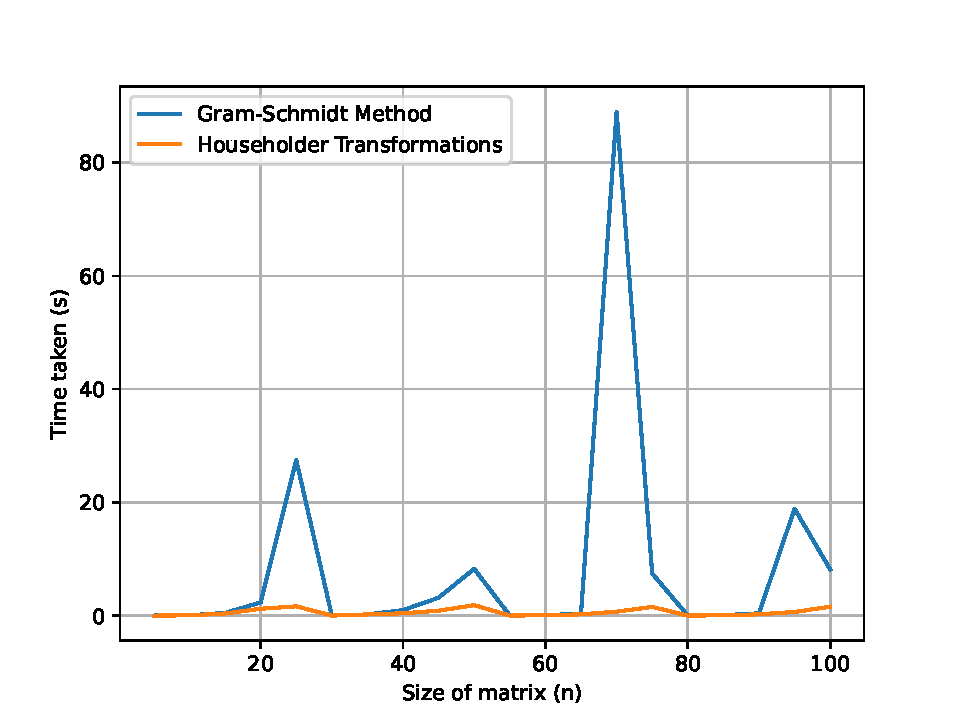
\includegraphics[width=0.5\textwidth]{../figs/compare}
    \caption{Performance comparison between Gram-Schmidt and Householder implementations}
\end{figure}

The performance of the Gram-Schmidt implementation varies a lot based on the matrix.
For some matrices it takes 20-30 times as much time as other matrices. Due to this
inconsistency, the Householder implementation is preferred.

The performance of the Householder implementation was measured for matrices of size
up to $n = 250$. The data was collected using \texttt{householder250.sh} into
\texttt{data/householder250.dat}, after which \texttt{plot.py} was used to plot the data.

\begin{figure}[h!]
    \centering
    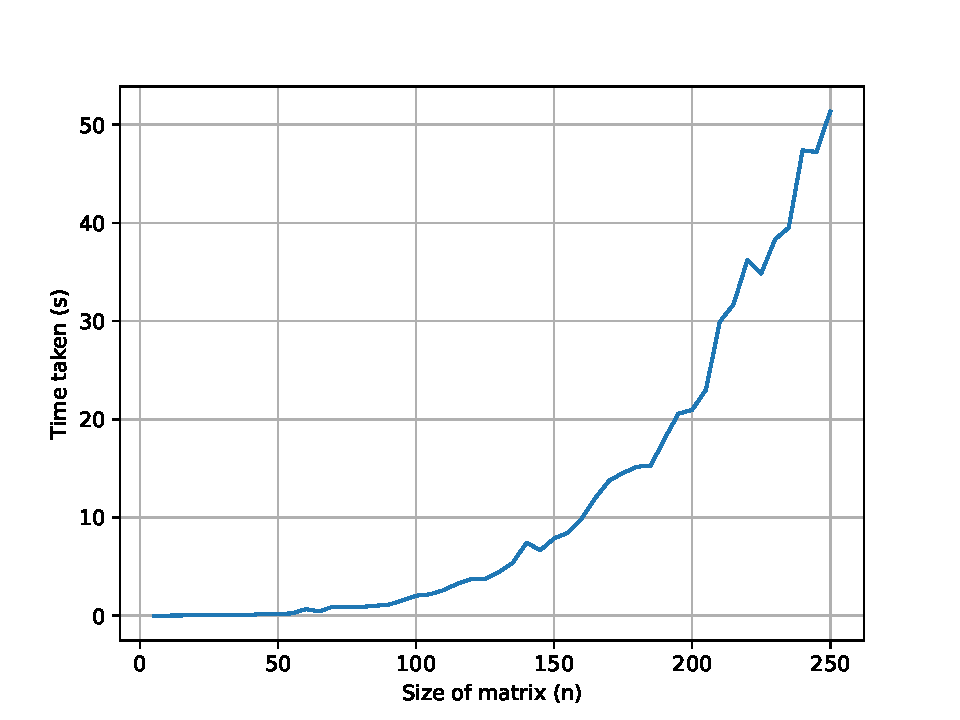
\includegraphics[width=0.5\textwidth]{../figs/householder250.pdf}
    \caption{Performance of the Householder implementation for large matrices}
\end{figure}

\section{Conclusion}

Thus, we have implemented an algorithm to compute all the eigenvalues of
an arbitrary $n \times n$ matrix using the Gram-Schmidt process and
Householder transformations. Of these two, Householder transformations were found
to be more reliable. We also optimized our algorithm using techniques such as
shifts and deflation, leading to a significant performance incrrease.

In the future, further optimization methods such as Hessenberg reductions and
Givens rotations could be explored, as they might be a faster and more accurate way to
decompose the matrix.

Overall, working on this project provided valuable insights into various
aspects of linear algebra and matrix theory, and introduced me to the
inner working of scientific computing libraries such as NumPy, LAPACK
and eigen.h.

\nocite{*}
\printbibliography

\end{document}
